% !TEX root = ../my-thesis.tex
%

\chapter{Introduction}
\label{sec:introduction}

%\cleanchapterquote{Un petit chapitre pour le doctorant, un grand chapitre pour l'humanité}{Doctorant anonyme}{(Citation temporaire)}

\newV{Cette thèse s'inscrit dans le cadre du traitement d'images médicales 3D. Elle traite d'analyse d'images dans lesquelles les propriétés des structures d'intérêt découlent directement ou indirectement de considérations anatomiques. Dans cette thèse, les structures d'intérêt proviennent d'acquisition de vaisseaux sanguins.}

\newV{Lors de la segmentation des vaisseaux, il est courant d'utiliser comme étape préliminaire des filtres de rehaussement angiographique. Ils permettent de faciliter la segmentation en faisant ressortir les vaisseaux présents dans les images. Toutefois, le gain de performance obtenu par ces filtres par rapport à la segmentation globale est rarement évalué. Dans cette thèse, nous proposons donc de développer des outils d'analyse de tels filtres, puis d'évaluer les performances de ces filtres dans un cadre reproductible.}

Dans cette introduction, nous décrivons le contexte global de la thèse ainsi que ses principaux apports.

\section{Contexte global}
% quelques chiffres pour saisir l'importance du foie

\newV{Le foie participe à de nombreuses fonctions vitales telles que la digestion, l'élimination des déchets ou la gestion de la glycémie. Les maladies liées au foie sont responsables de deux millions de morts par an \cite{Asrani2019_liver_deseases}. On estime à un million le nombre de morts par complications dûes à la cirrhose, une maladie liée à l'apparition de tissus fibreux dans le foie. Un second million de décès est lié à une inflammation aigüe ou chronique du foie, l'hépatite, ainsi qu'au cancer du foie (carcinome). La consommation régulière d'alcool est une des causes principales de la cirrhose et de l'hépatite chronique. La cirrhose et le cancer du foie sont les $11^{ème}$ et $16^{ème}$ causes de mortalité à travers le monde.}

Dans ce contexte, le diagnostic et le suivi des maladies du foie sont des objectifs cruciaux pour les médecins. Les techniques d'imagerie non invasives ont considérablement révolutionné ces deux tâches en permettant d'observer l'anatomie interne des patients sans avoir recours à la chirurgie. Pour le foie, deux types d'imagerie sont particulièrement utilisés, la tomodensitométrie (TDM) et l'imagerie par résonance magnétique (IRM). 

\newV{La tomodensitométrie, inventée par Hounsfield en 1972 permet de mesurer l'absorption de rayons X par les tissus du patient. Cette acquisition se fait par coupes successives et permet de reconstruire de manière numérique une représentation 3D des organes. L'IRM repose sur un autre principe physique qui utilise le champ magnétique. La première machine IRM permettant l'acquisition d'un corps humain a été développée en 1977 par Damadian. Lors d'une IRM, on mesure le temps de précession des tissus, c'est-à-dire le temps de changement de leur orientation magnétique après une exposition brève et intense à un champ magnétique. Cette acquisition, elle aussi réalisée par coupes successives, permet d'obtenir un volume 3D des organes. Le fonctionnement détaillé de la TDM et de l'IRM est explicité dans ce manuscrit en section \ref{sec:contexte:images}.}  

\newV{L'observation des vaisseaux sanguins présente des difficultés supplémentaires pour ces deux modalités, car l'intensité des vaisseaux peut se fondre dans les tissus environnants, rendant impossible tout diagnostic. Pour résoudre ce problème, on utilise des agents de contraste.
Pour la tomodensitométrie, on utilise des agents à base d'iode qui absorbent en quantité importante les rayons X. Des agents à base de gadolinium sensibles au magnétisme sont utilisés pour l'IRM. L'agent de contraste est injecté par voie intraveineuse lors de l'acquisition des images. Dans le foie, un nombre important d'échanges sanguins ont lieu. Le radiologue doit donc estimer correctement le temps de propagation du produit de contraste. Si l'image est acquise trop tôt, l'agent de contraste n'a pas le temps de se répandre dans le réseau vasculaire. Si l'image est acquise trop tard, l'agent de contraste se répand dans la totalité de l'organe le rendant opaque ; toute visualisation des vaisseaux devient alors impossible. On réalise en général plusieurs acquisitions (avant, pendant et après injection) de manière à fournir un maximum d'informations au radiologue.}

Les deux techniques d'imagerie sont complémentaires. La tomodensitométrie offre une grande résolution spatiale et permet de visualiser plus finement les détails, mais elle souffre d'un contraste entre les tissus plus faible. Au contraire, l'IRM possède une plus grande résolution de contraste, mais avec une résolution spatiale plus limitée que la TDM. C'est le médecin radiologue qui a la charge de choisir la méthode la plus appropriée. Pour les vaisseaux du foie, les deux systèmes sont utilisés. \newV{On peut toutefois noter qu'en pratique, les médecins essaient d'exposer le moins possible un patient à un examen à risque tel que le rayonnement ionisant émis par la tomodensitométrie}. Il y a donc une utilisation croissante de la tomodensitométrie à faible dose de rayons X et de l'IRM, moins agressive par rapport à la tomodensitométrie. Ces images sont cependant plus difficiles à exploiter et l'extraction automatique des vaisseaux pour visualiser les réseaux vasculaires nécessite des algorithmes de plus en plus performants.


\section{Présentation du projet ANR}
\label{sec:introduction:objectifs}
% Présentation du projet ANR

Cette thèse fait partie du projet R-Vessel-X\footnote{\url{http://tgi.ip.uca.fr/r-vessel-x/}} lancé en janvier 2019 et porté par Antoine Vacavant. R-Vessel-X a pour objectif l'extraction de vaisseaux sanguins du foie dans les images biomédicales dans le but d'assister les médecins pour la planification opératoire. \newV{Un point clé du projet est de proposer des algorithmes robustes dont la conception s'appuie sur les points suivants :}

\begin{itemize}
\item \newV{la capacité des modèles utilisés à prendre en compte les changements de tailles, de formes et d'intensités pour représenter et extraire les vaisseaux ;}
\item la fidélité des segmentations par rapport aux données originales et la possibilité de corriger celles-ci par les médecins ;
\item la validation des solutions développées grâce à des mesures effectuées sur des données synthétiques, cliniques et un retour de médecins ;
\item la dissémination des algorithmes et des données du projet afin d'assurer une pérennité de ces travaux et une réutilisation par la communauté.
\end{itemize}

Le projet R-Vessel-X rassemble des acteurs de la recherche publique ainsi qu'un partenaire industriel. Quatre laboratoires de traitement d'images ont apporté des compétences qui leur sont propres. Le LIRIS de l'Université de Lyon et le LORIA de l'Université de Lorraine apportent leur expertise sur l'analyse d'images par géométrie discrète et contribuent à développer la recherche reproductible. Le CReSTIC de l'Université de Reims Champagne-Ardennes est spécialisé dans l'analyse d'images médicales, la simulation et la visualisation 3D. Enfin, l'Institut Pascal de Clermont-Auvergne apporte son expertise sur l'analyse et la segmentation des vaisseaux sanguins du foie. 

Tout au long de cette thèse, nous avons pu collaborer avec ces différentes structures en partageant des données et des vérités terrains. Nous avons aussi partagé des jeux de données dont les vaisseaux ont été rehaussés afin qu'ils soient incorporés dans des algorithmes de segmentation.

Afin de juger de la qualité des algorithmes de segmentation, et en particulier leur adéquation avec une utilité clinique, deux radiologues du CHU de Clermont-Ferrand ont rejoint le projet. Ils ont aussi eu la charge de collecter des données nécessaires au projet.

\newV{Enfin l'entreprise Kitware Inc. spécialisée dans le développement d'outils pour l'imagerie médicale a fourni un appui technique au projet. Nous nous sommes en effet reposé sur leurs outils de compilation (CMAKE) et leur librairie de traitement d'images médicales (ITK) pour concevoir nos algorithmes. De plus, Kitware a proposé l'aide de deux de ses ingénieurs afin d'intégrer les algorithmes du projet à ses logiciels existants.}

\newV{Nous avons ainsi pu participer, en collaboration avec les radiologues, à l'élaboration d'un plug-in d'annotation et d'extraction des vaisseaux au logiciel de visualisation 3DSlicer qui intègre nos travaux sur le rehaussement de vaisseaux. Cet outil open source permet d'assurer une visibilité et surtout une utilisation internationale des algorithmes du projet.}

%\begin{figure}[ht]
%    \centering
%    
\includegraphics[height=6cm]{Images/labs.png}
%    \caption{Structures participant au projet ANR R-Vessel-X.}
%    \label{fig:labs}
%\end{figure}

% Apports de la thèse
\section{Résumé de la thèse et apports}
\label{sec:introduction:résumé}

Cette thèse est dirigée par Bertrand Kerautret, professeur au LIRIS, et Nicolas Passat, professeur au CReSTIC. Elle est co-encadrée par Odyssée Merveille, maître de conférences au laboratoire CREATIS. 

\newV{
L'objectif initial de cette thèse était la segmentation des vaisseaux du foie dans des images 3D. La segmentation des vaisseaux sanguins dans cet organe reste un problème ouvert. En effet, les vaisseaux hépatiques sont des structures dont le nombre de voxels est faible par rapport à l'ensemble de l'image. De plus, ils sont difficilement détectables par leur apparence bruitée et faiblement contrastées en plus d'être des structures fines, dont la taille peut approcher les limites de la résolution des images.}
\newV{Au demeurant, la littérature qui concerne la segmentation des vaisseaux hépatiques est plus réduite que pour d'autres organes (cerveau, cœur, fond d'œil 2D, etc.), en particulier pour la segmentation 3D et la segmentation IRM. La même observation est valable pour les jeux de données proposant une vérité terrain des vaisseaux hépatiques.}

\newV{Un premier objectif a donc été d'identifier des briques algorithmiques de méthodes de segmentation capables d'exploiter la géométrie 3D des vaisseaux. Les briques choisies devaient être robustes aux artefacts caractéristiques de l'imagerie du foie et ne pas demander un besoin excessif en annotations (i.e. méthodes d'apprentissage). La famille des filtres de rehaussement de vaisseaux semblait remplir ces conditions.}
\newV{
Ces filtres ne sont pas des méthodes de segmentation, mais bien des méthodes de filtrage qui interviennent en amont de celle-ci. Ils permettent notamment de faire ressortir les structures tubulaires, et donc les vaisseaux, dans des contextes diversifiés (Fig. \ref{fig:enhancement_example}). La littérature concernant ces filtres est variée avec une dizaine de filtres apportant des solutions à différentes problématiques du filtrage des vaisseaux sanguins.} Pourtant, une analyse plus fine de la littérature montre qu'en pratique, la plupart des chaines de segmentation utilisent l'un des premiers filtres proposés : le filtre de Frangi \cite{Frangi1998_vesselness}. De plus, dans la plupart des articles, ce filtre est utilisé avec les paramètres par défaut suggérés par Frangi en 1998, sans étudier si cette paramétrisation est adéquate pour la tâche concernée.


\begin{figure}
  % Frangi
  \centering
  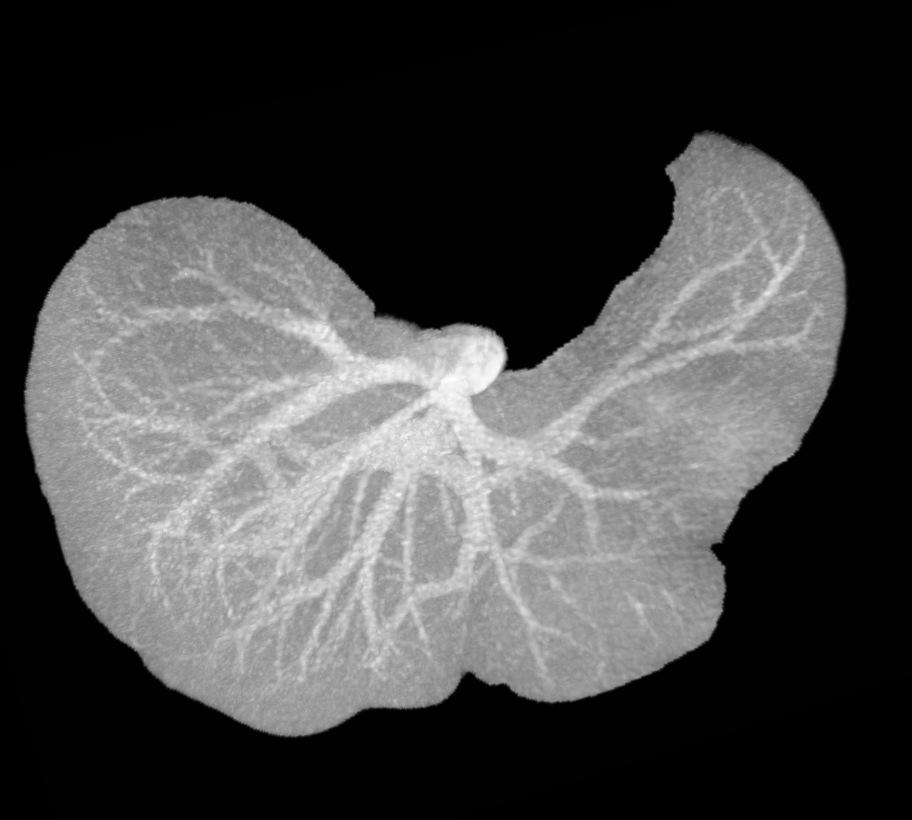
\includegraphics[clip = true, trim  =  10 150 10 150, width=0.46\textwidth]{Images/Ircad_original_volume.png}
  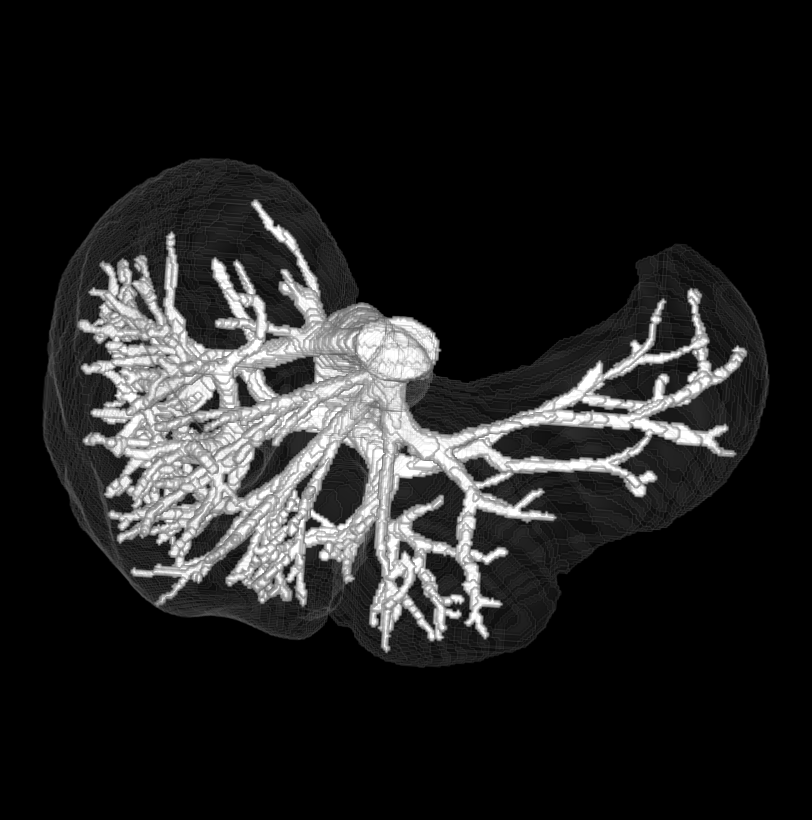
\includegraphics[clip = true, trim  =  10 150 10 150, width=0.46\textwidth]{Images/Ircad_GT.png}
  \\
  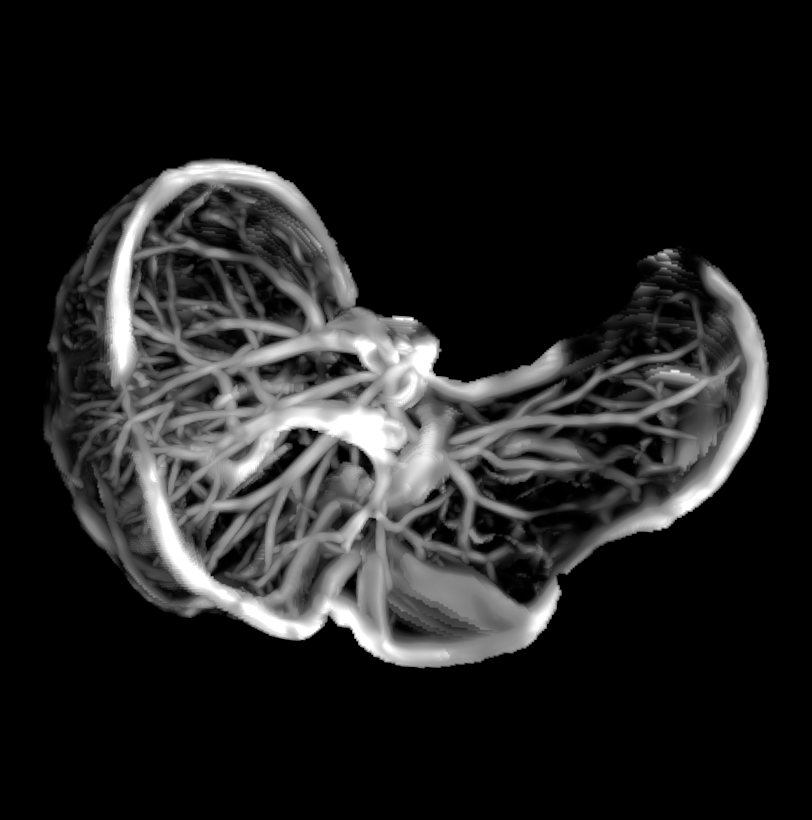
\includegraphics[clip = true, trim  =  10 150 10 150, width=0.46\textwidth]{Images/Ircad_Frangi.png}
  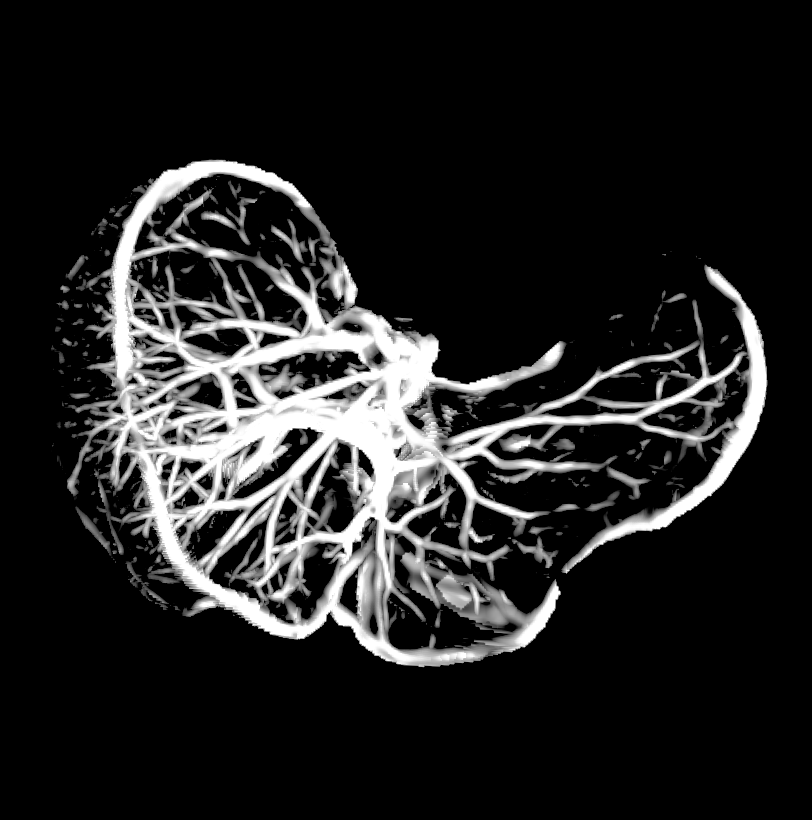
\includegraphics[clip = true, trim  =  10 150 10 150, width=0.46\textwidth]{Images/Ircad_Jerman.png}
  \caption{Image du foie en TDM et deux exemples de rehaussement. De gauche à droite et de haut en bas : image originale, vérité terrain, filtre de Frangi et filtre de Jerman.}
  \label{fig:enhancement_example}
  \end{figure}

On peut donc légitimement se poser plusieurs questions. Le filtre de Frangi est-il le filtre le mieux adapté pour toutes les tâches de rehaussement de vaisseaux ? Est-ce qu'un filtre est plus adapté à une modalité particulière ? Les filtres plus récents proposent-ils un rehaussement de meilleure qualité ? Quel est l'impact réel de la paramétrisation des filtres sur le rehaussement final ? \newV{Comment se comportent ces filtres pour l'imagerie du foie ?}

Malheureusement, les bancs de test qui étudient seulement la qualité du rehaussement de vaisseaux, \newV{sans étapes additionnelles de segmentation,} sont peu nombreux et non extensibles. Leurs travaux ne peuvent donc pas être repris, soit parce que le code original n'est pas disponible, soit parce que les données ne sont pas publiques ou les deux en même temps. \newV{En adéquation avec la philosophie du projet R-Vessel-X nous avons proposé les contributions suivantes :}

\begin{itemize}
\item la collecte, l'implémentation et la mise à jour en C++ d'une sélection de filtres de rehaussement parmi les méthodes développées ces vingt dernières années. Chacun de ces filtres illustre une réponse à une problématique distincte du rehaussement de vaisseau ;
\item un outil de comparaison de méthodes de rehaussement modulable permettant de comparer le rehaussement dans des zones spécifiques définies par l'utilisateur ;
\item une analyse quantitative poussée de ces filtres en fonction de la hiérarchie des vaisseaux définie par leurs tailles ainsi que de zones spécifiques comme les bifurcations ;
\item une analyse qualitative liant le choix des paramètres des méthodes à la réponse théorique des filtres et leur impact sur le rehaussement ;
\item une démonstration en ligne permettant de tester les filtres et leurs paramètres sans installation préalable et sur ses propres données ;
\item un outil d'annotation spécialisé pour la segmentation des vaisseaux du foie, ainsi qu'une série de bases de données publiques retravaillées pour répondre au manque de données annotées.
\end{itemize}

Ce travail a été réalisé dans un esprit de partage pour la communauté. C'est pourquoi une attention particulière a été apportée pour que ces travaux puissent être réutilisés et étendus par d'autres chercheurs, afin que ceux-ci n'aient pas à commencer leurs expériences à partir de zéro.

Ce manuscrit est organisé en \chapTotal{} chapitres : 

\begin{itemize}
\item Le chapitre \chapContextN{} présente le contexte clinique et scientifique de cette thèse. Celui-ci détaille l'anatomie du foie et présente les deux méthodes principales pour acquérir des images de manière non invasive ainsi que les différents artefacts liés à cette acquisition. Enfin, il introduit les bases de données publiques et leur intérêt dans le contexte de cette thèse.

\item Le chapitre \chapSOTAN{} introduit le rehaussement de vaisseaux. \newV{Il commence par résumer les contraintes pratiques liées à la visualisation des données médicales, et notamment le rôle de la segmentation dans la visualisation 3D. Il présente ensuite les méthodes principales de segmentation afin de comprendre de l'utilité du rehaussement}. Il explique enfin les concepts sur lesquels repose le rehaussement de vaisseaux : les espaces multi-échelles et les caractéristiques de tubularité. Les espaces multi-échelles permettent de capturer les structures de l'image de différentes tailles tandis que la caractérisation de la tubularité permet de ne sélectionner que les vaisseaux.

\item Dans le chapitre \chapBenchN, nous discutons de la construction d'un banc de test afin d'évaluer les filtres de rehaussement. Ce chapitre décrit également les traitements des jeux de données nécessaires à l'évaluation des filtres et les choix qui ont guidé les principes de fonctionnement de cet outil.

\item Le chapitre \chapAnalysisN{} illustre l'utilisation de ce banc de test par une analyse des performances de sept filtres de rehaussements à travers cinq jeux de données différents (TDM, IRM et trois jeux d'IRM synthétique). Cette analyse étudie à la fois les performances des filtres les uns par rapport aux autres et l'influence de leur paramétrisation sur le résultat final de manière quantitative et qualitative. L'évaluation est menée sur le rehaussement au niveau de l'organe, du voisinage des vaisseaux de différentes tailles et de leurs bifurcations. 

\item Nous discutons ensuite dans le chapitre \chapReproN{} de la reproductibilité de nos travaux ainsi que du travail mené pour promouvoir leur diffusion. Cette diffusion passe par la valorisation de nos travaux par des publications en journaux et en conférences, mais aussi par le développement de démonstrateurs et de plug-ins pour un logiciel de visualisation 3D.

\item Enfin, le chapitre \chapEndN{} propose des perspectives liées au rehaussement ainsi qu'un bilan de nos travaux. Nous montrons en particulier l'intérêt du rehaussement pour les méthodes de segmentation populaires de nos jours, ainsi qu'une ouverture sur la segmentation des vaisseaux à partir de la seule annotation des bifurcations.
\end{itemize}
    